\chapter{Introduction}
\label{Introduction}

Phages are small viruses on the order of 27-190nm that infect and lyse (kill) specific bacteria, acting as nature's natural anti-microbial defense. 
Researchers are attempting to determine how phages can be used in various medical and industrial applications to control bacterial growth. 
However, researchers need to know how the interactions between phages and bacteria work in order to implement a robust method to control bacterial growth. 

\section{Thesis Overview}
This thesis covers multiple topics to ultimately answer how phages and bacteria interactions can be mathematically modelled. 
First, there is a (biological) introduction to phages and bacteria. 
This introduction covers how phages work and infect bacteria, how bacteria defend against phages, how phages defeat bacterial defenses, and how phages defend against other phages. 
There is also an introduction to different modelling techniques such as spatial vs non-spatial models and ODEs vs DDEs. 
This thesis briefly covers software that models phages, resources, bacteria, and their limitations. 

This thesis presents software I developed to support the research, demonstrating its capabilities using a representative model of phage-bacteria-resource interactions. 
The section also provides an overview of its usage, including example outputs from demonstration runs.
Finally, the results generated by the software will be thoroughly analyzed and discussed.

\section{Biological Background}
Phages are small viruses on the order of 27-190nm (the average size of marine phages are 54nm) that infect and lyse (kill) specific bacteria.
Phages are so small, that it takes 55 million phages to cover the period at the end of this sentence \cite{breitbartPhagePuppetMasters2018}. 
The phage cycle process starts with a phage coming into contact with a bacterium.
Once it has identified an injection site, the phage can inject a strain of DNA into the bacteria.
The DNA strand has two options: it can either merge into the bacterial DNA, allowing the phage's DNA strand to replicate alongside the bacteria as they reproduce.
This process defines the Lysogenic cycle.
After a set amount of time, the DNA of the phage can unmerge and hijack the DNA replicating mechanism, creating multiple copies of itself, using the transcription, translation, and replication process to create multiple copies of itself.
The phages begin to self-assemble inside the bacteria until the bacteria is full of phages and explodes, the lysis stage, releasing the phages into the environment, ready to repeat the process again. 

This process can be visualized in \Cref{fig:phage_life_cycle}.
\begin{figure}
    \centering
    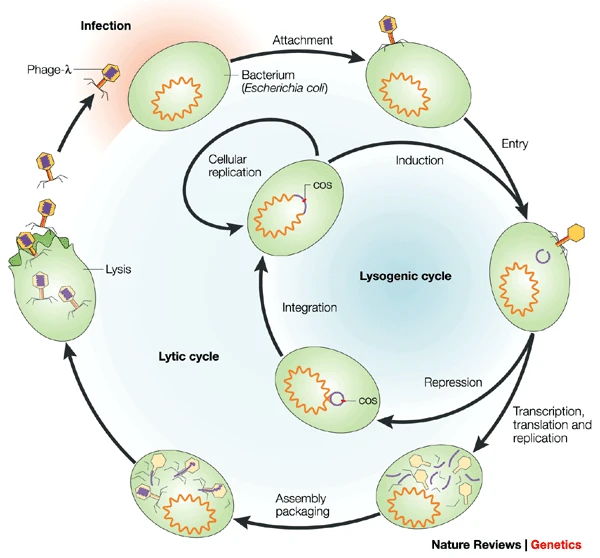
\includegraphics[width=0.5\linewidth]{Figures/phage_life_cycle.png}
    \caption{Life cycle of a phage, inside and outside a bacteria cell. Significant steps in the life cycle of a phage include the infection stage, integration, replication, and lysing process. Figure sourced from \citet{campbellFutureBacteriophageBiology2003}. }
    \label{fig:phage_life_cycle}
\end{figure}

\section{The Environment}
In an ecosystem like the ocean, the gut, or in soil, there are thousands of different microbes all interacting with one another or the surrounding environment.
The interactions are complex, with many factors affecting the growth of bacteria, phages, plants, animals, and more. 

The interactions between agents in the environment are often synergistic. 
When an animal dies, bacteria start to digest and decompose the animal into simpler chemicals like carbon and nitrogen that plants can use to grow, which is then eaten by other animals. 
External factors, such as flooding, droughts, chemical spills, or introduction of new agents have a massive impact on the ecosystem. 
These events can add or remove resources from the system, change environmental parameters such as the surrounding temperature, introduce competition, or create an imbalance in the population by killing agents. 
These effects have a larger effect on the ecosystem and food chain as a whole as bacteria are one of the fundamental foundations for resource recycling. 

\subsection{Phage's Role in the Environment}
Phages play a large role in the ecosystem. 
As bacteria die, for example through lysis, they release resources into the environment for other bacteria and plants to use. 
This turns over resources like nitrogen and carbon for other sources to use. 
Phages also help mediate horizontal gene transfer, disperse pathogenic diseases, and spread antibiotic resistance \cite{al-shayebCladesHugePhages2020}. 
Phages directly alter bacteria population diversity and population fitness by introducing new ways for bacteria to mutate \cite{brownEcologicalFunctionalRoles2022}. 
There are about $10^6$ bacteria cells/ml and $10^7$ phages/ml of marine water. 
About 5\% of any bacteria are currently infected and about 15\% of daily bacterial death can be attributed to phages \cite{chibani-chennoufiPhageHostInteractionEcological2004}. 


Phage populations depend on growth by infection and death by degrading. 
UV is a large factor of killing marine phages, causing up to a 5\% reduction in phage infectivity per hour \cite{chibani-chennoufiPhageHostInteractionEcological2004}. 

\subsubsection{Phages and Controlling Bacterial Blooms}
Phages could potentially be used to control \textit{Cyanobacteria} (blue-green algae) blooms in the environment \cite{colomaFrequencyVirusresistantHosts2019}. 
\textit{Cyanobacteria} cause damage to aquatic life by consuming resources and oxygen, starving aquatic life and negatively affect human health. 
There is hope that phages can be used to biologically control water quality in waste water treatment plants and in the environment without the use of harsh chemical processes what would otherwise pose environmental and health hazards \cite{krysiak-baltynSimulationPhageDynamics2017, tuckerIdentificationCyanophageMaLBP2005}. 
More information about controlling \textit{Cyanobacteria} can be read in \nameref{sec:AppendixB:environmental_protection}. 

\section{Phage Cocktails and Human Health}
There is particular interest in phage applications in human and animal health, called phage cocktail therapy, due to phage cocktails not exhibiting side effects.
Phage cocktails are a medicine that sick patients with bacterial diseases, such as \textit{Escherichia coli} can use. 
A patient can swallow a pill filled with a range of different phages that target \textit{E. coli}.
The phages will target the specific \textit{E. coli} bacteria, but it will not affect the other bacteria found in the gut of the human body and will not have any side effects on the body. 
There are about 100 trillion microbes across 5,000 different types of bacteria strains in the human gut. 
Antibiotics disrupt the intricate ecosystem of the gut microbiome, acting as a scorched-earth mechanism. 
Phages on the other hand specifically target a specific bacterial strain, acting as a sniper, with minimal to no effects to other bacterial strains, while antibiotics act as a bomb. 
A challenge that antibiotics face is that antibiotics create antibiotic resistant bacteria, making the antibiotic less effective in the future \cite{odonkorBacteriaResistanceAntibiotics2011, volkovaEffectsEarlylifePenicillin2021}. 
There is however hope that phage resistant bacteria become more susceptible to antibiotics due to changes in the cell structure \cite{laurePhageResistancemediatedTradeoffs2022, zhaoPhagedrivenCoevolutionReveals2024}. 
\nameref{sec:AppendixB:phage_therapy_and_antibiotics} in \nameref{AppendixB} goes more in depth on how phages can be used in a healthcare setting. 

\section{Industrial Usage}
Phages have many uses in an industrial setting. 
Similarly, phage therapies can be used as a preventative method, by preventing the spread of common bacteria in livestock by dosing the animal feed with the phage pills. 
Farmers often raise livestock in tight spaces with a lack of sanitation facilities, increasing the risk of a disease spreading. 
 
Phages can be used to control the growth of bacteria like \textit{Salmonella} while producing food in a factory \cite{sofferBacteriophagesSafelyReduce2016, kowalskaFreshVegetablesFruit2023}. 
\nameref{sec:AppendixB:controlling_foodborne_bacteria} in \nameref{AppendixB} goes into more detail about using phages to control foodborne bacteria. 

\section{Modelling Phages in a Complex Community}
Not much is known about phages in large and complex communities between other phages, bacteria, resources, and the environment. 
There have been previous attempts to model the complex dynamics of the populations between phages, bacteria, and resources, with the environment using Ordinary Differential Equations (ODE) and Delay Differential Equations (DDE).
Not every interaction in the complex community can be identified, and if an interaction has been identified, the associated parameter values are unknown and need to be experimentally derived. 
Collecting interaction parameter values is an expensive and laborious task, as the data has to experimentally collected. 

There are two main ways to model phage-bacteria dynamics: spatially and non-spatially.
In a spatial model phages and bacteria can move through space and interact with their neighbors. 
Partial differential equations (PDE) and cellular agent-based models (ABM) have been used to model spatial interactions.
Spatial models require special considerations, such as proximity to other agents.
This creates areas of interaction and interest where agents are located, and areas of no interactions where there are no interactions.
Spatial models lead to more computationally complex models, but can result in more interesting and biologically realistic results. 

Whereas in non-spatial models such as ODEs and DDEs, the bacteria and phages are assumed to be in a well-mixed solution and no distinctions are made in regard to neighbors or distances to other agents. 
Interactions are simplified to a probabilistic approach, where a percentage $p$ of agents interact with one another at time step $t$.
Non non-spatial models are easier to develop, understand, and are more effective in modeling large populations, at the cost of losing spatial information. 

For this thesis, the focus will be modelling resource, phage, and bacteria interactions using an ODE model. 
A phage-bacteria-resource system is described as an $p\times b \times r$ system, meaning $p$ phages, $b$ bacteria, 
Current modelling methods have mainly stayed with $1\times 1 \times 1$ models, meaning 1 phage, 1 bacteria, and 1 resource. 
This thesis aims to develop a simulation framework that can model any $p\times b \times r$ ODE system, where each agent can contain states (called hidden agents) that they can move to and from. 
\newline 

\section{Software Overview}
The project is divided into three logical parts, with an optional fourth part.
The first section is to create the network interaction. 
Here the user of the software can define the number of resources, phages, and bacteria, who interacts with who, and the strength and type of interactions. See \nameref{sec:network_creation_tool} for further information. 
In \nameref{sec:simulation_framework}, the user uploads the network model and parameters and as output receives the time data and population data as an array. 
\nameref{sec:visualization_framework} allows the user to interact with \nameref{sec:network_creation_tool} and \nameref{sec:simulation_framework} with a dashboard. 
The user can graphically edit the attribute values of the edges and nodes of the network, and the user can run more advanced visualizations, for example by changing a parameter value and seeing how that affects the population count. 
There are a few plots included out of the box that the user can test. 
The plots offered in part 3 offer interactivity like hiding and showing lines and dots, zooming in and out, and hovering over the lines and dots to show more details of the data. 

Finally, the user can optionally run multiple simulations and download the data to their disk to create their own custom visualizations using \nameref{sec:custom_visualizations_and_framework}. 
The visualizations created in \nameref{sec:visualization_framework} can theoretically be recreated in \nameref{sec:custom_visualizations_and_framework}. 
The user can choose the same parameter values used for a specific plot in \nameref{sec:visualization_framework}, run the simulation (under the \nameref{sec:ultimate_analysis} section), download the data, and reimplement the graphs. 

The user can use the tool themselves by importing the Python classes in their own code and initializing the classes and passing the appropriate data. 